%!TEX root = Thesis_main.tex

\chapter{Experimental Setup}
\label{chapter6}

The Mobile Manipulator under analysis in this thesis is a prototype assembled at the University of Southern California in the Center of Advanced Manufacturing (CAM) Laboratory. The system has been called ADDAMS (Agile  Dexterous  Autonomous  Mobile Manipulation System) and it is shown in Figure \ref{imgADDAMS1}.

\begin{figure}[h!] 
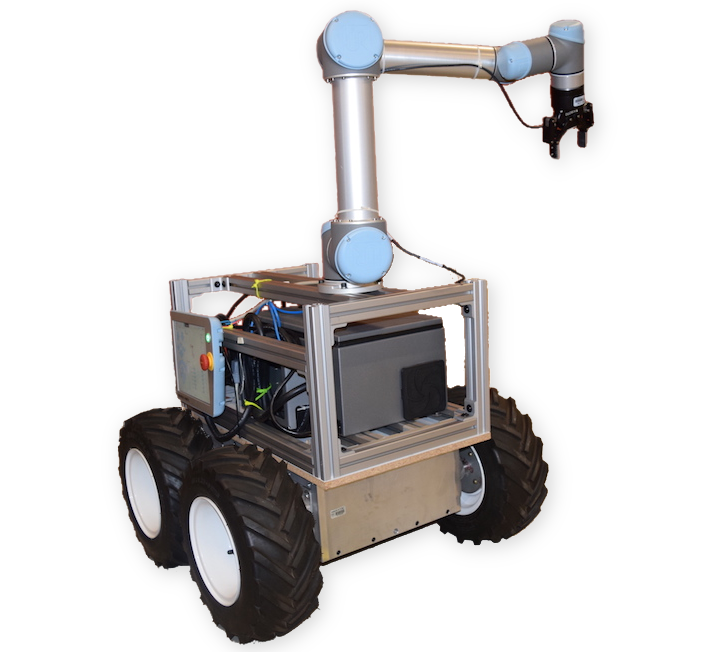
\includegraphics[scale=0.25]{ADDAMS1}
\centering
\caption{ADDAMS}
\label{imgADDAMS1}
\end{figure}

The goal of this prototype is to study a system able to handle parts as well as to perform operations in unstructured industrial environments to fill the gap between small and large production systems. Indeed, companies with small production volumes are nowadays required to innovate production systems towards the generation of smart factories. Given that those companies are generally not economically able to manage automated production lines and that the production mix is generally changed frequently, flexible systems to support production are required. For those reasons ADDAMS wants to be a low-cost solution, using low-cost sensors and to be capable, once its operation has been planned, to perform tasks in any environment. \\


The controller presented in this thesis wants to be the first step towards the design of an online software that makes the system able to operate autonomously once the task has been given. In the next sections the main components of ADDAMS will be shown in its Hardware and Software parts; then setups used for simulations and physical tests will be presented. 
\section{Hardware}

\subsection{Mobile Base}

\begin{figure}[h]
\begin{center} 
	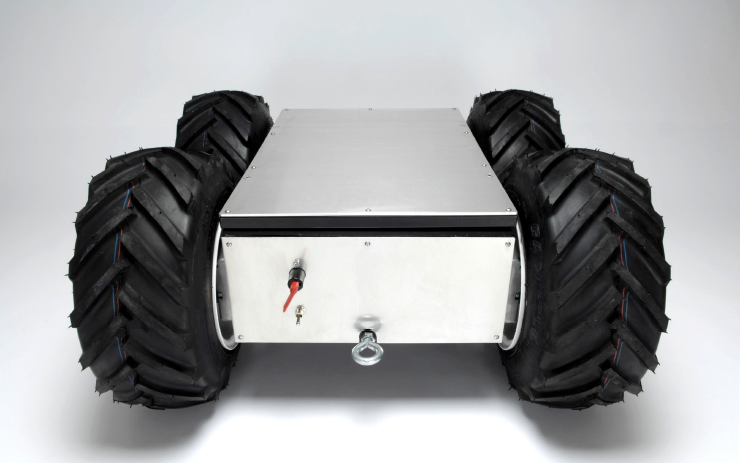
\includegraphics[scale=0.6]{SuperMegaBot1}
	\centering
	\caption{Nonholomic Mobile base}
	\label{fig:SuperMegaBot1}
\end{center}
\end{figure}
The mobile base shown in Figure \ref{fig:SuperMegaBot1}, provided by InspectorBots and named Super Mega Bot (SMB), is a Heavy-Duty, All-Terrain, 4WD robotic platform. It is a rugged, indoor/outdoor platform and can be fitted with a variety of sensors, cameras and equipment. The base has been designed to be Modular and Reconfigurable, so an end user can swap out various modules. There are several methods available provided by the manufacturer to control the SMB including RC radio, Analog Joystick, Wireless Modem, or Microcomputer.\\
The SMB is designed with non-steering coupled wheels and because of that the rotation of the base is obtained giving different velocities to the right and left wheels. For this reason, the SMB is configured as a differential-drive mobile robot for which the kinematic relationships explained in Chapter \ref{chapter2} hold. This particular mobile platform has been chosen for its high payload and because it is large enough to keep on its upper surface the UR5 control unit. In Appendix \ref{AppA} technical data of the SMB and information about the motors used can be found.

\subsection{UR5 Manipulator}
The UR5 is a collaborative robotic arm developed by Universal Robots. According to the company, the key benefits of their robots are lightweight, safety and easiness to use. The robotic arm is regarded as safe because it will stop acting as soon as the robot hits an object sensed by a force sensor in one of the joints. UR5 is ideal for automating low-weight processing tasks like picking, placing and testing. The medium-sized robot arm is easy to program, fast to set up and, always according to UR, offers one of the fastest payback times in the industry. Because it is designed as a collaborative robot, the UR5 is generally suitable for tasks in which the operative space of the robot is shared with humans and that fits also ADDAMS objectives. The UR5 comes from the manufacturer with its control unit that can be easily accessed and provides low-level controllers for tracking velocities of the joints. More technical details on UR5 can be found in Appendix \ref{AppB}.

\begin{figure}[htbp]
\begin{center} 
	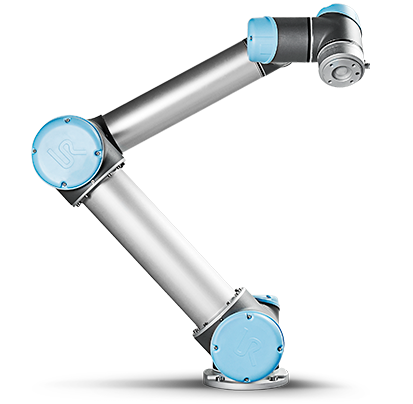
\includegraphics[scale=0.4]{UR5}
	\centering
	\label{fig:UR5}
	\caption{UR5 robot arm} 
\end{center}
\end{figure}


\subsection{Sensors}

The sensors of the ADDAMS prototype are used to measure the positions of the joints, in order to perform the desired task. Briefly, the sensor system is composed of:
\begin{itemize}
\item angular encoders for the UR5 joints, which provide an accuracy of $0.1$ mm at the end effector position;
\item encoders on the wheels of the base, that will be used to derive the position and orientation of the mobile base through a simple transformation.
\begin{equation*}
\begin{split}
\theta_b=&T\frac{r(\omega_R-\omega_L)}{d} \\ x_b=T\frac{r(\omega_R+\omega_L)}{2}\cos\theta_b &\qquad y_b=T\frac{r(\omega_R+\omega_L)}{2}\sin\theta_b
\end{split}
\end{equation*}
This measuring system is reliable only at slow speed and provides an accuracy of $\pm 2$ cm. Since the position of the end effector is computed knowing the position of the base, the accuracy of these measures is not sufficient to perform precise operations. Considerations on this aspect will be done later on.
\item a lidar that can be used to measure unknown obstacles position in the operative area of the robot.
\item a Kinect sensor for Simultanous Localization And Mapping (SLAM)
\end{itemize}

\section{Software}

To easily interface with all the components of ADDAMS we used ROS, an open-source, meta-operating system for robotic systems. ROS provides the services that allow communication between all the components, message-passing between processes, hardware abstraction, low-level device control. It also provides tools and libraries for obtaining, building, writing, and running code across multiple computers. The ROS network used to run the physical system is shown in the graph of Figure \ref{ROSnodes}
\begin{figure}[h!]

\makebox[\textwidth][c]{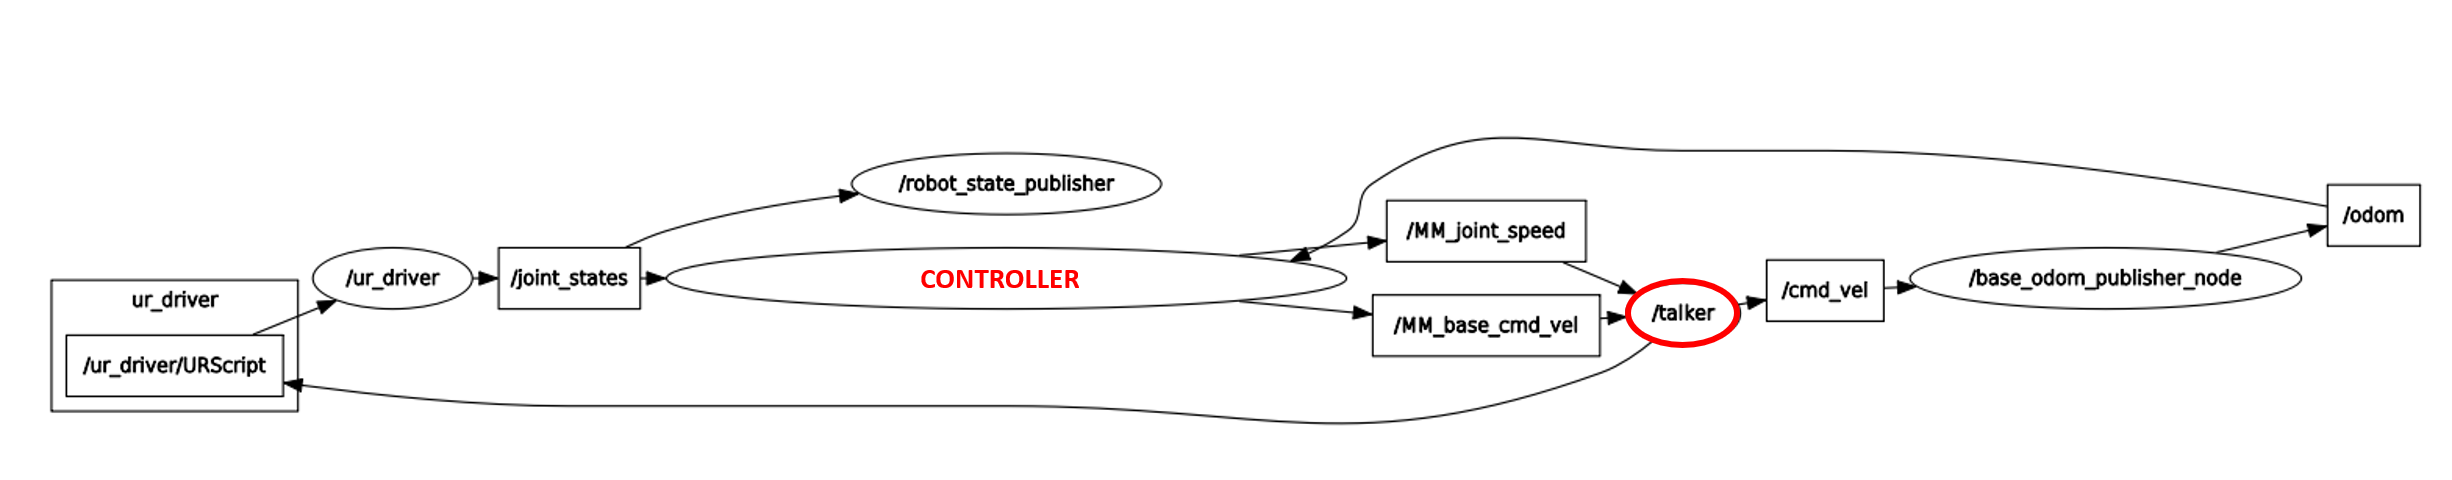
\includegraphics[scale=0.4]{nodegraph1}}
\centering

\caption{ROS nodes and messages for ADDAMS}
\label{ROSnodes} 
\end{figure}

The controller we designed has been developed using Matlab/Simulink environment through CasADi, an open-source tool for nonlinear optimization and algorithmic differentiation that allows using Matlab/Simulink to define optimization problems and different commercial solvers. More information about CasADi can be found in \cite{Andersson2018}. The solver used to solve the Nonlinear Problem described in Chapter \ref{chapter5} is IPOPT; a brief introduction to IPOPT can be found in Appendix \ref{AppC}. As shown in the graph of Figure \ref{ROSnodes}, the Simulink node where the controller is running, reads position of the base and joint angles and give velocity commands to the system through a "talker" node we defined to communicate with the robot. As already mentioned, the commands given to the system are velocity commands, i.e. high-level commands that the system is required to track. Anyway, given that the manufacturers already provides reliable low-level controllers able to track those desired velocities, we decided to use, as mentioned in Chapter \ref{chapter5}, a hierarchical approach that is briefly explained in Figure \ref{Hdiagram}.  
\begin{figure}[h!]

	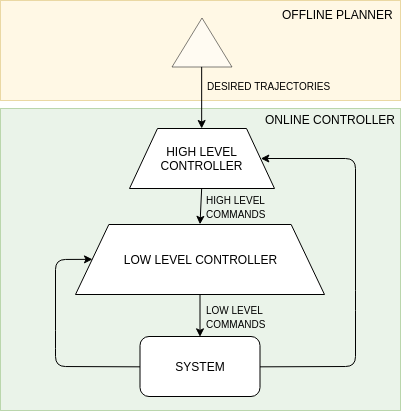
\includegraphics[scale=0.5]{Hdiagram}
	\centering
	
	\caption{Control hierarchy} 

\label{Hdiagram}
\end{figure}
\\
Simulations and physical experiments have been carried out to test the developed controller and to analyze performances and influences of parameters. In particular two tasks have been tested: 

\begin{itemize}
\item \textbf{Movement of the system toward/from the grasping area}. Referring to the controller as presented in Chapter \ref{chapter5} we will consider the cost function expressed in Equation \ref{costfunctionh} as a composition of $h_4$ and $h_5$. Indeed, the task of moving the system towards the grasping area is performed controlling the base and joint angles positions without requiring to track the end effector position. The choice of this formulation for the cost function allows the problem to be easier to solve given that we are tracking joint angles rather than compute through Forward Kinematics the EE position. Furthermore, the arm is generally not required to move during the movement of the system.

\item \textbf{Trajectory tracking inside grasping area}. In this case we will consider the problem of tracking the EE position considering the cost function \ref{costfunctionh} as a composition of $h_1$, $h_2$ and $h_3$, and eventually $h_4$ in the cases when the base is required to not stop. This task is more of interest for this thesis and then will be discussed more in detail. Considerations about online changing the cost function will be given in the next chapter. 
\end{itemize}
\section{Simulations setup}

Simulations for both the tasks object of study have been performed using Simulink to test stability, robustness, performances and effects of the parameters on the controller. The model used to simulate the system is basically the same presented in Chapter \ref{chapter2}, computing the state of the system through numerical integration. The block diagram in Figure \ref{simdiagram1} shows the simple architecture of the controller used in simulations.

\begin{figure}[h!]
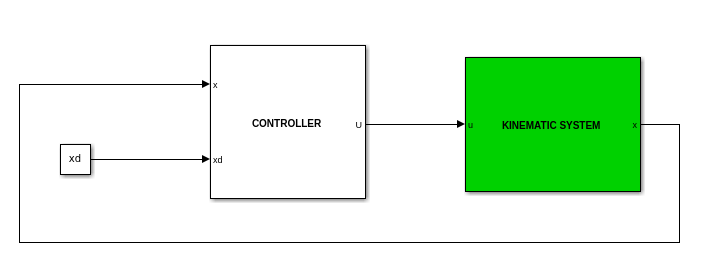
\includegraphics[scale=0.45]{simdiagram1}
\centering
\caption{Simulations block diagram} 
\label{simdiagram1}
\end{figure}

The results of the simulations have been saved and processed in MATLAB R2018b. The solver for the optimization problem (IPOPT), as shown in Chapter \ref{chapter5} works at a given frequency $f_c=\frac{1}{T_k}$. Each time the solver is called, as we see in Equation \ref{ourproblem_param_vinc}, four terms are needed to compute a new control action: 
\begin{itemize}
\item $x_{k|0}$: the state measured at time instant $k$, used as a starting point to propagate the future states;
\item ${x_{k|i}}_d \ \ \forall i=1,\dots,N$: the desired states for the control horizon;
\item $u_{k-1|0}$: needed to compute the velocity constraint at time step $i=0$;
\item $p_0$: the initial guess of the parameters to be estimated solving the problem.
\end{itemize}
Referring to this last term $p_0$, the value has been chosen, both for simulations and physical experiments, equal to zero at the initial time (i.e. a vector of zeros). For all the other calls of the solver $k\neq0$, the previous optimal solution $p_{k-1}^*$ has been given. This choice generally helps to find the solution faster, given that the previous solution is usually not so far from the new one.
\begin{figure}[h!]
	
	\makebox[\textwidth][c]{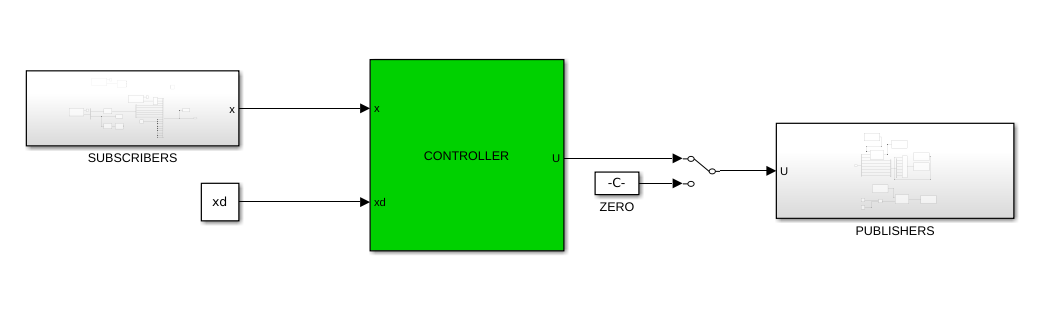
\includegraphics[scale=0.4]{diagramreal}}
	\centering
	
	\caption{Physical experiments block diagram} 
	
	\label{diagramreal}
\end{figure}
\section{Physical Experiments Setup}
The software setup for the physical experiments, as anticipated, makes use of ROS to interface with the real system. In particular, the controller node has been created in Simulink by means of the Robotic System Toolbox provided by Mathworks. The control input velocities have been given to the system by means of a communication node to interface with the low-level controllers. Figure \ref{diagramreal} shows the architecture of the controller used for Physical experiments.



%Performances of the low-level controller have been tested primarily giving step input velocities commands to test the response of the base and the arm joints. In Figure \ref{testllbase} and \ref{testllarm} are reported the step responses of the base linear velocity $v$ and the joint angle velocity $\dot{\Theta}_3$ respectively.
%\begin{figure}[ht]
%\centering
%\subfigure[Base step response]{%
%\label{testllbase}%
%
\includegraphics[scale=0.15]{empty}}%
%\qquad
%\subfigure[Arm joints step response]{%
%\label{testllarm}%
%
\includegraphics[scale=0.15]{empty}}%
%\caption{Low level controllers step response}
%\end{figure}
%The measurements of the performed velocity for these tests have been derived from joints encoders for the arm and encoders on the wheels for the base. Since the main aim of the low-level robot controllers is to track some velocity profile, after testing the step response, the tracking of a simple sine trajectory has been analyzed. In Figures \ref{testllbase2} and \ref{testllarm2} are reported the results.
%\begin{figure}[ht]
%\centering
%\subfigure[Base sine response]{%
%\label{testllbase2}%
%
\includegraphics[scale=0.15]{empty}}%
%\qquad
%\subfigure[Arm joints sine response]{%
%\label{testllarm2}%
%
\includegraphics[scale=0.15]{empty}}%
%\qquad
%\subfigure[Base tracking error]{%
%\label{testllbase3}%
%
\includegraphics[scale=0.15]{empty}}%
%\qquad
%\subfigure[Arm joints tracking error]{%
%\label{testllarm3}%
%
\includegraphics[scale=0.15]{empty}}%
%\caption{Low level controllers trajectory tracking}
%\end{figure} \\
%The errors with respect to those trajectories are shown in \ref{testllbase3} and \ref{testllarm3}. We can see that the responses show an overdamped behaviour. Indeed, robot low-level controllers are always overdamped, although the ideal case will be a critically-damped system.  If the system would be underdamped the behaviour of the system can lead to overshoots that are generally not desired in robotic applications. At the same time if the system is too much overdamped the robot movement becomes very sluggish. Hence most controllers are designed to give a near critically-damped response.